\documentclass{article}
\usepackage[margin=1.25in]{geometry}
\usepackage{amsmath, amssymb, setspace, enumerate, enumitem}
\usepackage{setspace}
\usepackage{graphicx}
\onehalfspacing

\begin{document}
    \begin{enumerate}
        \item \begin{enumerate}[label=(\alph*)]
            \item Two items will have high cosine similarity if they are pointing in roughly the same direction $\approx 1$, and they will have high Euclidean distance similarity if their points are far from each other.\\[0.25in]
            Two vectors parallel to each other, pointing at the same direction, and are close to each other, will have high cosine similarity and low Euclidean distance similarity.\\[0.25in]
            Two vectors parallel to each other, pointing in the opposite direction, and are far from each other, will have low cosine similarity and high Euclidean distance similarity.
            \item Cosine similarity will change because if the origin changes, the angles will change as well. Euclidean distance similarity will remain the same as the distance between two vectors will not change when the origin is changed.
        \end{enumerate}

        \item Consider the two cases present:\\
        $\pi \geq \frac{1}{2}$, then $e(f(x)) = 1 - \pi(x)$, $\pi(x) \geq 1 - \pi(x)$ based on our condition.\\
        $\pi < \frac{1}{2}$, then $e(f(x)) = \pi(x)$, $\pi(x) < 1 - \pi(x)$ based on our condition.\\
        Then, it appears that $e(f(x)) = min\{\pi(x), 1 - \pi(x)\}$ depending on the value of $pi$, which is either $\geq \frac{1}{2}$ or $< \frac{1}{2}$.\\[0.25in]
        $f(x)$ is our target function, so there is no other hypothesis that has a smaller error other than the target function, we build our hypothesis to attempt to guess the target hypothesis.

        \item \begin{enumerate}[label=(\alph*)]
            \item The decision boundary for 1-NN, blue represents +1, red represents -1: \\ 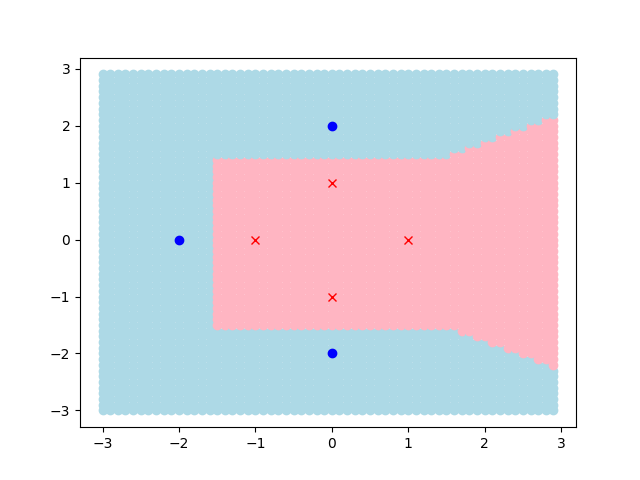
\includegraphics[scale=0.5]{images/p6_1_a.png}\\[0.25in]
            The decision boundary for 3-NN, blue represents +1, red represents -1: \\ 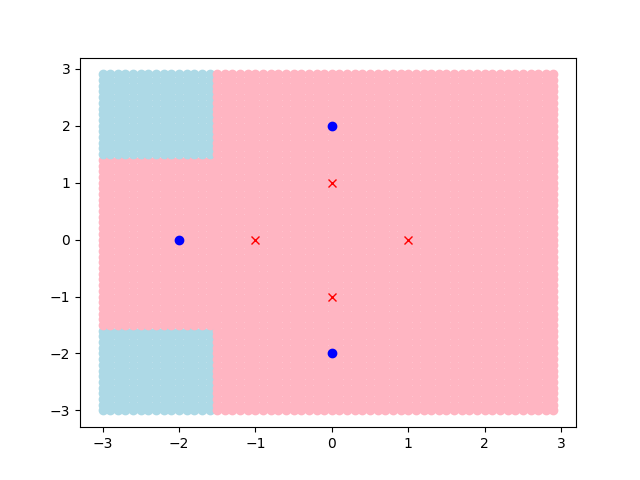
\includegraphics[scale=0.5]{images/p6_1_a_3.png}
            \item Decision boundaries are the same as previously mentioned, for 1-NN of the transformed dataset, we have \\ 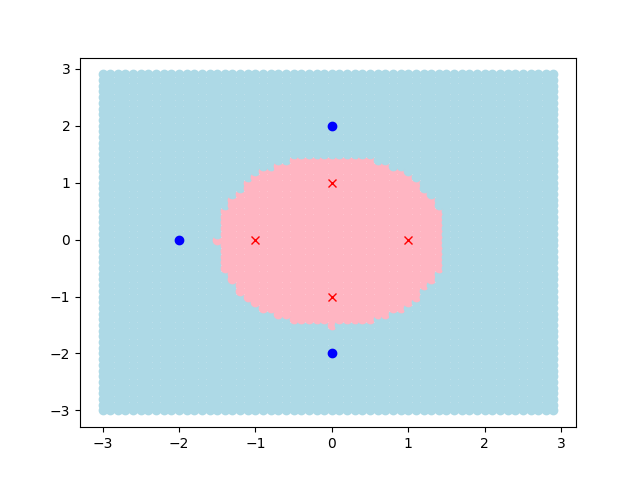
\includegraphics[scale=0.5]{images/p6_1_b.png}\\[0.25in]
            for 3-NN, we have \\ 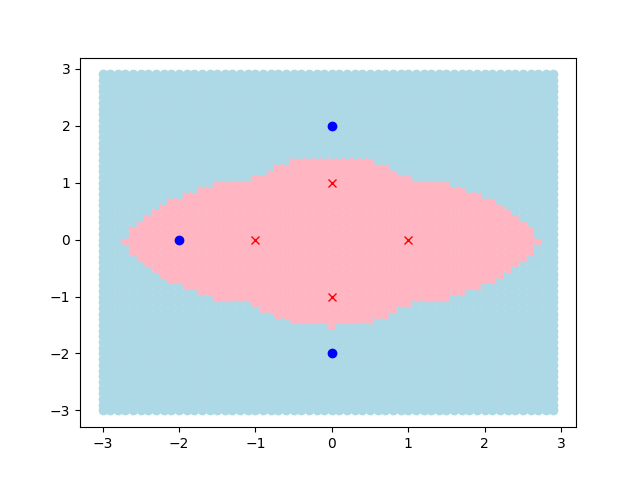
\includegraphics[scale=0.5]{images/p6_1_b_3.png}
        \end{enumerate}
        
        \item For the 1-NN case:\\ 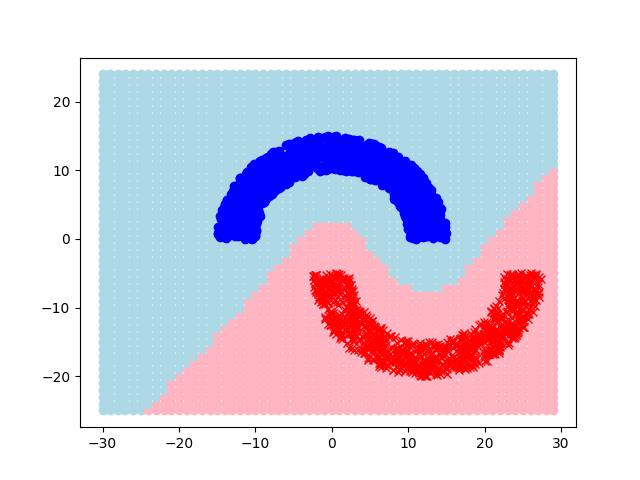
\includegraphics[scale=0.5]{images/6_3_1NN.png}\\[0.25in]
        For the 3-NN case:\\ 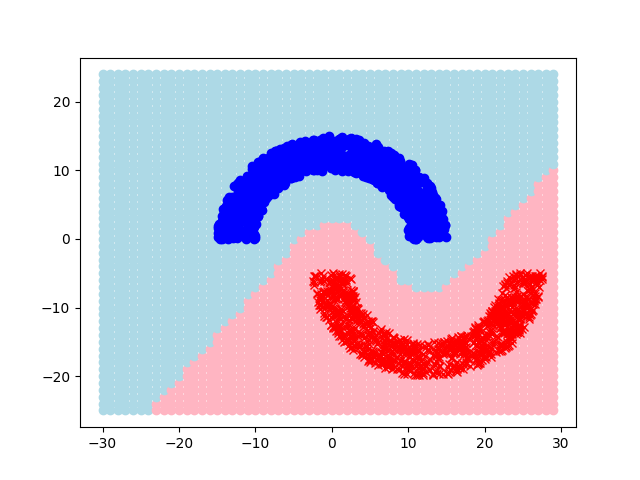
\includegraphics[scale=0.5]{images/6_3_3NN.png}\\[0.25in]
        Both grpahs seems similar.

        \item \begin{enumerate}[label=(\alph*)]
            \item The running time for the branch and bound was 34.82s, while the running for brute force was 114.75s, a large difference. It seems like ignoring entire partitions of data that are not necessary using the partitioning algorithm improves the time by around 3 fold, when the datapoints are $N = 10000$.
            \item With the gaussian centers, the runtime seems pretty identical, the branch and bound was 46.89s while brute force was 124.74s. The time significantly drops when I reduce $\sigma = 0.01$ instead of $\sigma=0.1$.
            \item I expected a lower runtime with the gaussian centers since the datasets should be more compact and clustered, but after running the algorithm, I think the scale $\sigma$ was too high at $0.1$, when I plotted the graph out, it seems like all the clusters were grouped tightly.\\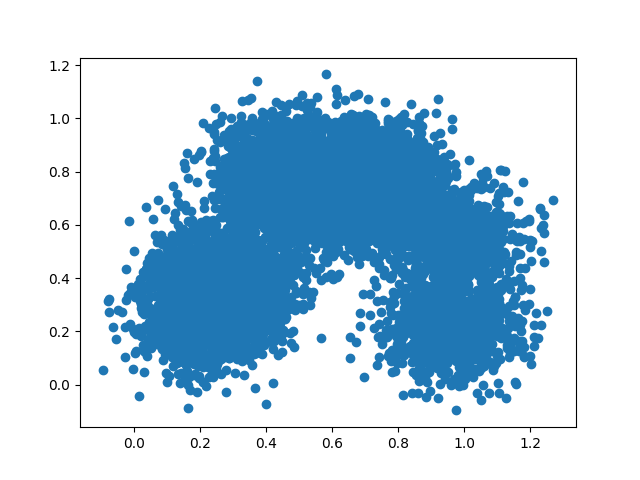
\includegraphics[scale=0.25]{images/p6_16_b.png}\\When running the branch and bound algorithm, we find the nearest neighbor in $S_1$ and continue looking at other partitions, we do the calculation to see if the nearest point in partition $S_j$ is less than our current nearest neighbor, if so, we look through all the points in that partition. But it appears that when partitions are this grouped together, we end up visiting perhaps more partitions as there exist points where the nearest neighbor requires us to go through every single partiton, thus failing the purpose of branch and bound.
            \item No. Only if it is a miniscule amount like $<100$ data points, which we can do quickly without branching and bounding. However, for any larger dataset (to be honest, every dataset you encounter will probably be large), it's always optimal to use branch and bound.
        \end{enumerate}
    \end{enumerate}
\end{document}